\section{Consensus layer support}

We will now start constructing a concrete blockchain proof protocol. Before
we're able to define the prover and the verifier algorithms, we need to propose
certain modifications to the consensus layer.

Knowing that the id of a block must be less than the mining target $T$ to
satisfy the proof-of-work condition, we observe that some blocks will achieve a
much lower id. If the block id is less than $\frac{T}{2^\mu}$ we say that the
block is of level $\mu$. Clearly all blocks are blocks of level $0$. Observe
then that in expectation, half of the blocks will be of level $1$, $1/4$ of the
blocks will be of level $2$, $1/8$ will be of level $3$ and so forth. We term
blocks that have a level above 0 \textit{superblocks} of their respective
level. Note that, in expectation, the number of superblock levels of a chain
$\chain$ will be $\log(\chain)$. The level of a block is formally given as $\mu
= \left \lfloor \log(T) - \log(\sf{blockid}(B)) \right \rfloor$.

Figure~\ref{fig.hierarchy} illustrates the blockchain superblocks starting from
level $1$ and going up to level $4$ in case these blocks are distributed
exactly according to expectation. Note that each level contains half the blocks
of the level below.

\begin{figure}[h]
    \caption{The hierarchical blockchain.
    Higher levels have achieved a lower target (higher difficulty) during mining.}
    \centering
    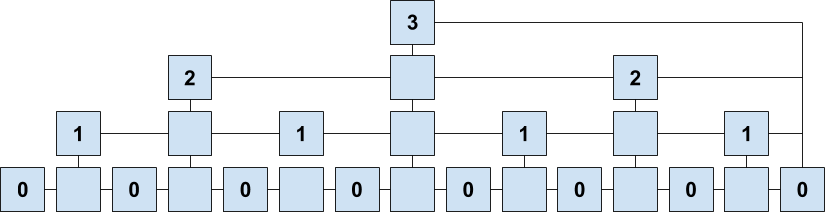
\includegraphics[width=0.5\textwidth,keepaspectratio]{figures/hierarchical-ledger.png}
    \label{fig.hierarchy}
\end{figure}

Some helper functions need to be defined. The \textit{blockid} function
calculates the id of a block given its data. This is done by applying the
hashfunctions $H$ and $G$ in a manner similar to \cite{backbone}:
$\textsf{id} = H(ctr, G(s, x, \textsf{interlink}))$. However, note that block
$B$ maintains an \textit{interlink} data structure instead of a previous block
pointer. We will get to this shortly. Note also that, while we spell out the
transaction vector $x$, this in practice contains only the root of the Merkle
tree of the transactins. We also define the \textit{level} function which
calculates the highest level of a block given its data.

The \textit{interlink} data structure is proposed to be included in each block,
replacing the existing pointer to the previous block with a list of pointers to
a small number of previous blocks. For each superblock level $\mu$, this data
structure contains a pointer to the most recent preceeding block of level
$\mu$. The algorithm for this construction is shown in
Algorithm~\ref{alg.nipopow-interlink} and is borrowed from \cite{KLS}. By
convention, we assume that the Genesis block is of infinite level and hence a
pointer to it is included in every block at the first available index within
the interlink data structure. For more information about the interlink data
structure, see \cite{KLS}. The interlink data structure turns the blockchain
into a skiplist-like data structure. Observe that the number of pointers that
need to be included per block is approximately $\log(\chain)$.

The updateInterlink algorithm accepts a block $B'$, which already has an
interlink data structure defined on it. The function then evaluates the
interlink data structure which needs to be included as part of the next block.
The algorithm proceeds by copying the existing interlink data structure and
then modifying some of its entries from level $0$ to the level of block $B'$ to
point to the block $B'$. Observe that the pointers stored are block ids and
hence block data needs to be looked up based on blockid. To this end, the full
node maintains a \textit{blockbyid} dictionary which, queried with the block
id, returns the block data. Finally, the full node also maintains a
\textit{depth} data structure which, given a block, returns its distance from
the Genesis block.

% \import{./}{algorithms/alg.nipopow-helper.tex}
\import{./}{algorithms/alg.nipopow-interlink.tex}
